\newpage
\section{提案手法}
本研究では,ハードウェア特徴点の採取システムを構築し,\fp~により端末構成を推定することを試みた.
これは既存の\fp~とは異なり,端末やブラウザを識別するだけではなく,端末がどのハードウェアで構成されているのかを明らかにするものである.
よって,ここでは新たに\hfp~という用語でこの手法を取り扱うこととする.
また,新たなハードウェア特徴点の採取法についても提案する.
\subsection{\hfp}
本研究では,\hfp~を\fp~を拡張して,``ブラウザ経由で採取したFingerprintにより端末の構成要素(ハードウェア)を識別する''と定義する.
\hfp~では,基本的に図~\ref{fig-hfp}で示すフローで推定を行う.これは一般的な教師あり学習であり,学習フェーズにてJavaScriptによる特定の演算結果をハードウェア情報でラベル付し教師データとする.そして,推定フェーズにて同様のJavaScriptによる演算を行った結果,教師データを参照して最も近しいラベルを推定結果とするものである.ここで重要なことは,教師データの確保である.すべてのハードウェアを推定するためには多くのハードウェア上で実行された演算結果があることが望ましい.また,ラベル付されたデータに統計的ではない間違いが存在すると著しく推定確度が低下することに留意しなくてはならない.
\begin{figure}[H]
	\centering
    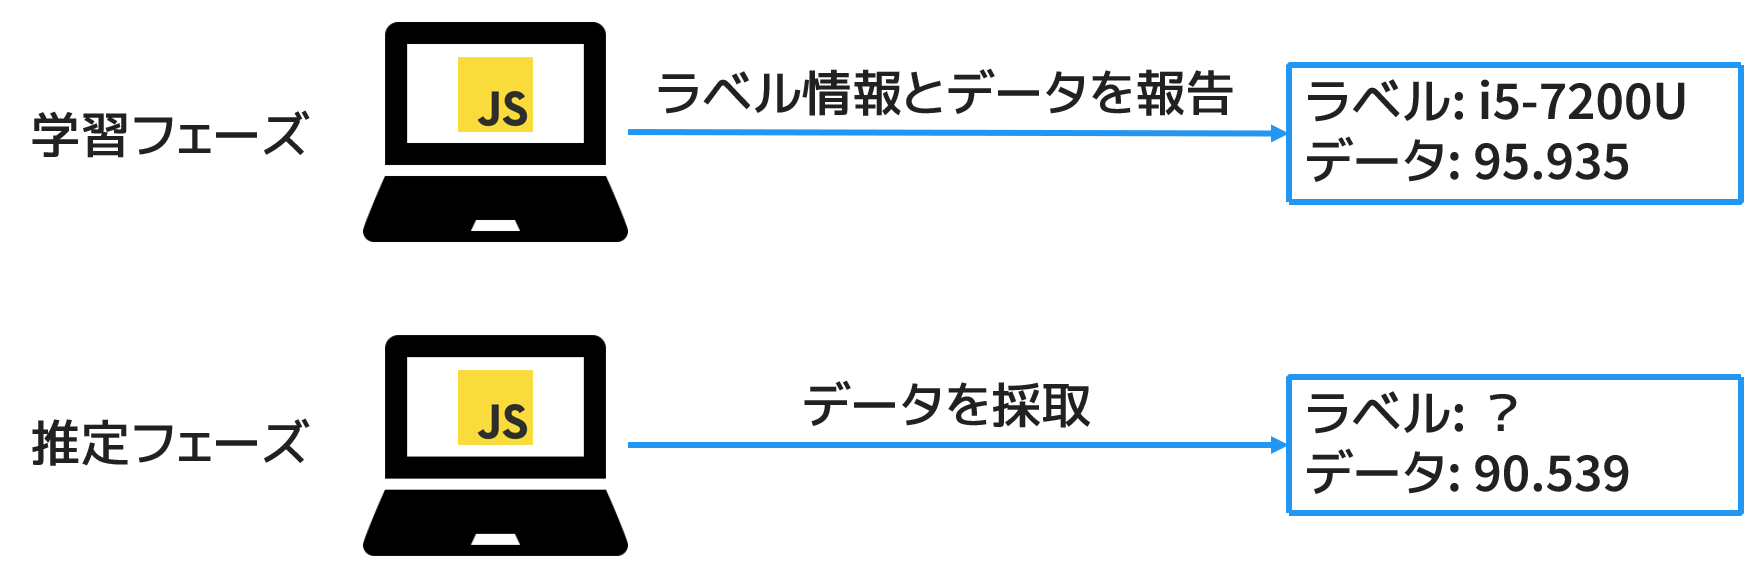
\includegraphics[width=\textwidth,pagebox=artbox]{fig/hfp.png}
    \caption{\hfp~の基本的なフロー}
    \label{fig-hfp}
\end{figure}
\subsection{\hfp~採取システム}
\begin{figure}[H]
	\centering
    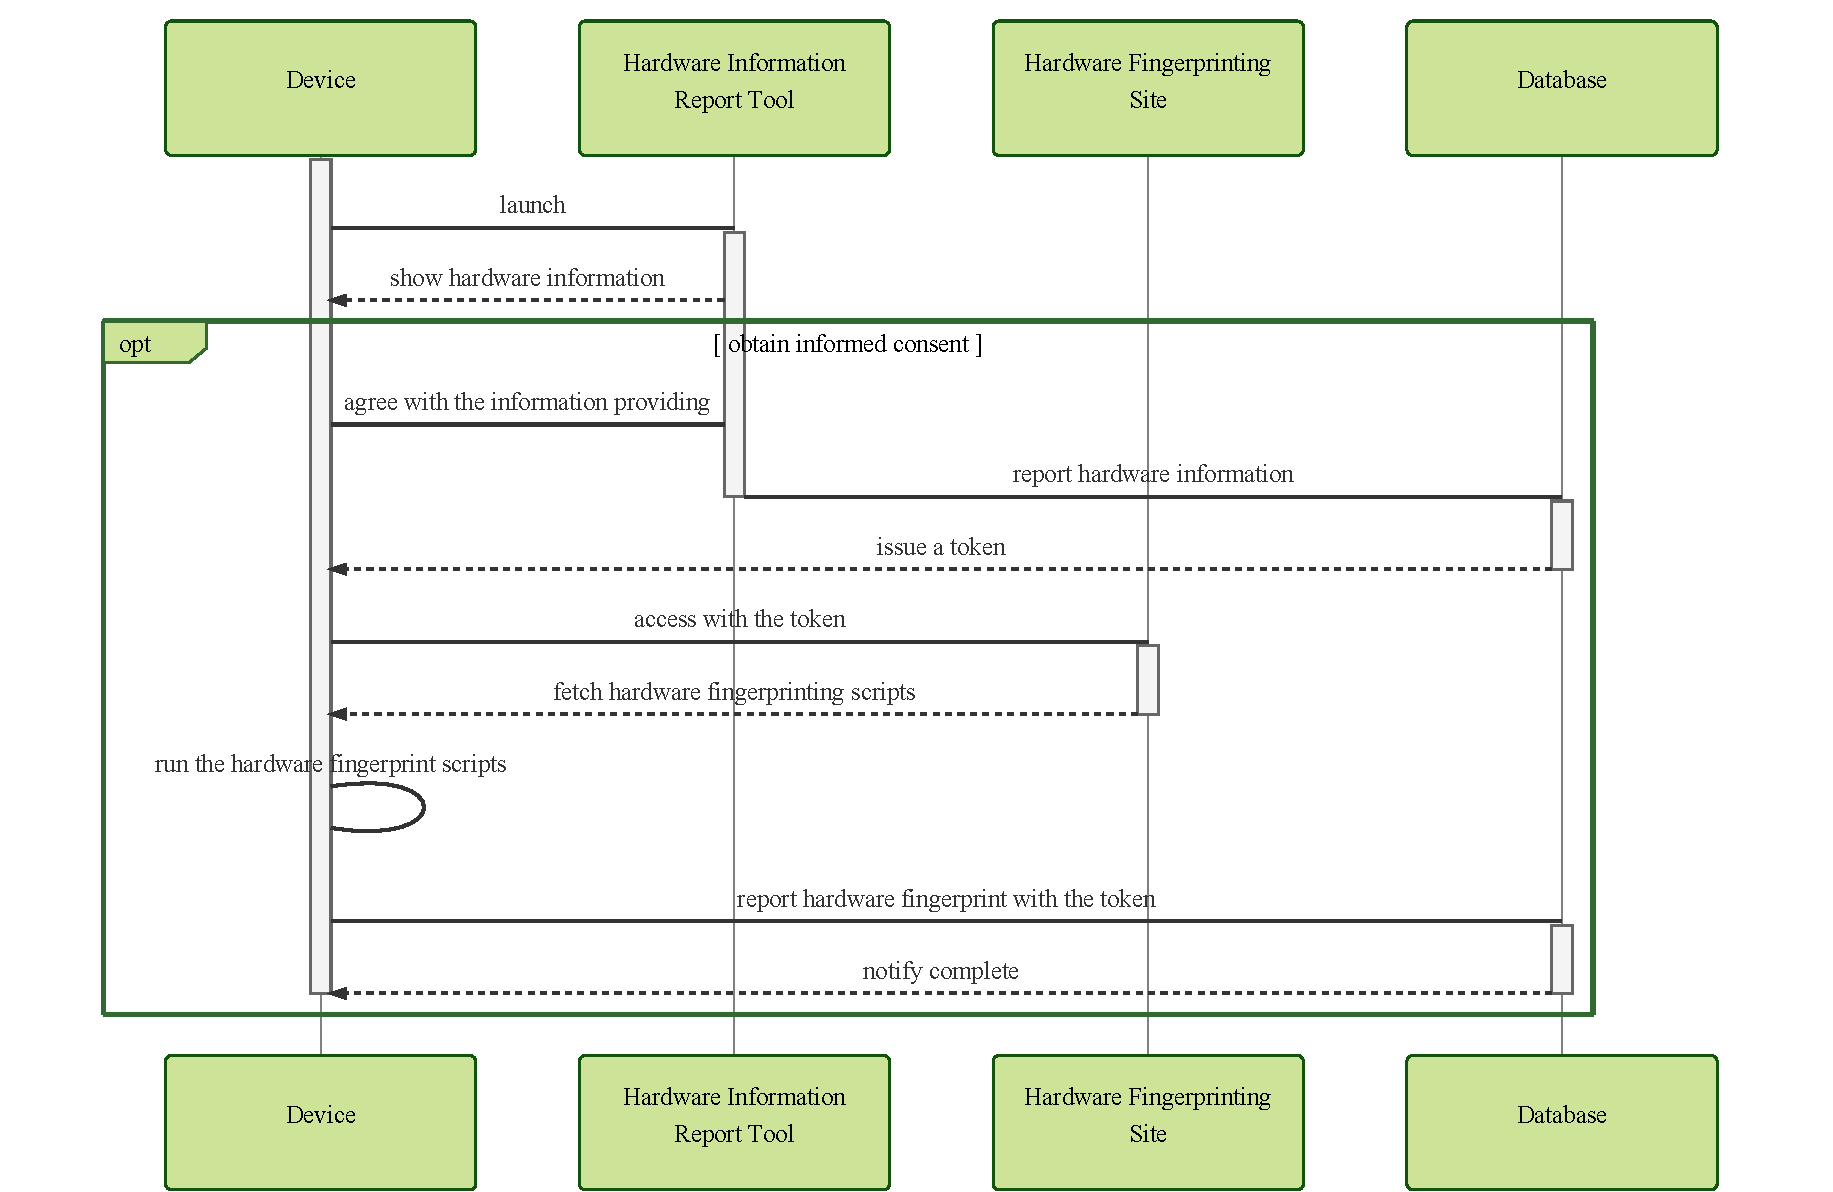
\includegraphics[width=\textwidth,pagebox=artbox]{fig/hero.pdf}
    \caption{\hfp~採取システムの流れ}
    \label{fig-hfp_system}
\end{figure}
\subsection{新たなハードウェア特徴点}
\subsubsection{AES-NI}
\subsubsection{Turbo Boost}
\subsubsection{CPUファミリ,マイクロアーキテクチャ,モデルナンバー}
\subsubsection{バイトオーダー}
\subsubsection{メモリのパフォーマンス}
\subsubsection{GPUのパフォーマンス}
